\documentclass[8pt]{beamer}
\usetheme{default} % Very simple theme
\usecolortheme{dove} % Minimalist grayscale colors
\setbeamertemplate{navigation symbols}{} % Remove navigation bar

% Define brand-like colors
\definecolor{myblue}{RGB}{0, 102, 204}    % Blue for standard blocks
\definecolor{mygreen}{RGB}{0, 153, 0}     % Green for example blocks
\definecolor{myred}{RGB}{204, 0, 0}       % Red for alert blocks
\definecolor{myorange}{RGB}{255, 128, 0} % For \emph

% Accent color for titles, bullets, etc.
\setbeamercolor{structure}{fg=myblue}

% Block colors
\setbeamercolor{block title}{bg=myblue, fg=white}
\setbeamercolor{block body}{bg=blue!5, fg=black}

\setbeamercolor{exampleblock title}{bg=mygreen, fg=white}
\setbeamercolor{exampleblock body}{bg=green!5, fg=black}

\setbeamercolor{alertblock title}{bg=myred, fg=white}
\setbeamercolor{alertblock body}{bg=red!5, fg=black}
\setbeamercolor{alerted text}{fg=myred}

% Optional: color for \example text
\setbeamercolor{example text}{fg=mygreen}

% Custom emph (orange text instead of italic)
\let\oldemph\emph
\renewcommand{\emph}[1]{\textcolor{myorange}{#1}}
\newcommand{\ve}[1]{\boldsymbol{#1}}

\usepackage{graphicx} % Package for images
\usepackage{amsmath} % Package for images
\graphicspath{{figs/}} % Path to your figures directory
\usepackage{array}  % For better column spacing
\usepackage{caption} % Required for \captionof

% Title Information
\title{STOCHASTIC METHODS IN WATER RESOURCES}
\vspace{25pt}
\subtitle{Unit 5: Geostatistics \\ Lecture 16: Generalities, descriptive spatial statistis}
\author{Luis Alejandro Morales, Ph.D.}
\institute{Universidad Nacional de Colombia \\ Department of Civil and Agriculture Engineering} %// }
%\date{\today}

\begin{document}

% Title Slide
\begin{frame}
    \titlepage
\end{frame}

%-------
% From Bierkens
\section{Generalities}
\begin{frame}{Generalities}
    \begin{itemize}
        \item \alert{Geostatistics} is the part of statistics that is concerned with \emph{geo-referenced data}, i.e. data that are linked to \emph{spatial coordinates}.
        \item To describe the \emph{spatial variation} of the property observed at data locations, the property is modelled with a \emph{spatial random function} (or \emph{random field}) $Z(\mathbf{x})$,  $\mathbf{x}^T = (x,y)$ or $\mathbf{x}^T = (x,y,z)$.
        \item The focus of geostatistics can be further explained by the figure below.
            \begin{center}
            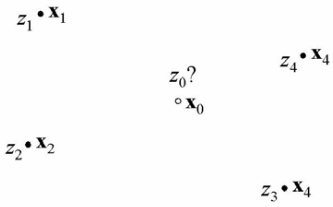
\includegraphics[width=0.6\linewidth]{fiBi71.png}  % from Bierk
            \end{center}
            Suppose that the values of some property (for instance \emph{hydraulic conductivity}) have been observed at the four locations $x_1$, $x_2$ , $x_3$ and $x_4$ and that, respectively, the values $z_1$ , $z_2$ , $z_3$ and $z_4$ have been found at these locations.
    \end{itemize}
\end{frame}

\begin{frame}{Generalities}
    \begin{itemize}
        \item \emph{Geostatistics} is concerned with the unknown value $z_0$ at the non-observed location $x_0$. In particular, \emph{geostatistics} deals with:
            \begin{enumerate}
                \item \emph{spatial interpolation and mapping}: predicting the value of $Z_0$ at $x_0$ as accurately as possible, using the values found at the surrounding locations (note that $Z_0$ is written here in capitals to denote that it is considered to be a \emph{random variable});
                \item \emph{local uncertainty assessment}: estimating the probability distribution of $Z_0$ at $x_0$ given the values found at the surrounding locations, i.e. estimating the \emph{probability density function} $f_z \left(z_0;\mathbf{x}_0 | z_1(\mathbf{x}_1), z_2(\mathbf{x}_2), z_3(\mathbf{x}_3)\right)$. This probability distribution expresses the uncertainty about the actual but unknown value $z_0$ at $\mathbf{x}_0$;
                \item \emph{simulation}: generating realisations of the \emph{conditional random function} $Z(\mathbf{x} | z(\mathbf{x}_i ), i=1,\cdots,4)$ at many non-observed locations $\mathbf{x}_i$ simultaneously (usually on a \emph{lattice} or \emph{grid}) given the values found at the observed locations; e.g. \emph{hydraulic conductivity} is observed at a limited number of locations but must be input to a groundwater model on a grid.
            \end{enumerate}
        \item \emph{Geostatistics} was first used as a practical solution to estimating ore grades of mining blocks (concentration or percentage of valuable minerals or metals within a block) using observations of ore grades that were sampled preferentially. i.e. along outcrops.Later it was extended to a comprehensive statistical theory for \emph{geo-referenced data}.
    \end{itemize}
\end{frame}
 
\begin{frame}{Generalities}
    \begin{itemize}
        \item Presently, \emph{geostatistics} is applied in a great number of fields such as \emph{petroleum engineering}, \emph{hydrology}, \emph{soil science}, \emph{environmental pollution} and \emph{fisheries}.
        \item Some important \emph{hydrological problems} that have been tackled using \emph{geostatistics} are among others: 
            \begin{itemize}
                \item spatial interpolation and mapping of rainfall depths and hydraulic heads;
                \item estimation and simulation of representative conductivities of model blocks used in groundwater models;
                \item simulation of subsoil properties such as rock types, texture classes and geological facies;
                \item uncertainty analysis of groundwater flow and -transport through heterogeneous formations (if hydraulic conductivity, dispersivity or chemical properties are spatially varying and largely unknown) 
    \end{itemize}
    \end{itemize}
\end{frame}

%-------
% From Bierkens
\section{Descriptive spatial statistics}
\begin{frame}{Descriptive spatial statistics}
    \begin{block}{Declustering}
    \end{block}
    \begin{itemize}
        \item Looking at figure above it can be seen that not all observation locations are evenly spread in space. Certain location appear to be \emph{clustered}. This can for instance be the case because it is convenient to take a number of samples close together.
        \item Another reason could be that certain data clusters are taken purposively, e.g. to estimate the \emph{short distance variance}.
        \item If the \emph{histogram} or \emph{cumulative frequency distribution} of the data is calculated with the purpose of estimating the true but unknown \emph{spatial frequency distribution} of an area, it would not be fair to give the same weight to \emph{clustered observations} as to observations that are far from the others. The latter represent a much larger area and thus deserve to be given more weight.
    \end{itemize}
    \vspace{-5pt}
\begin{minipage}[]{0.48\textwidth}
    \begin{itemize}
        \item To correct for the \emph{clustering effect declustering methods} can be used. Here, one particular \emph{declustering method} called \alert{polygon declustering} is illustrated in the figure.
        \item The figure shows schematically a spatial array of measurement locations. The objective is to estimate the \emph{spatial statistics} (\emph{mean}, \emph{variance}, \emph{histogram}) of the property (e.g. \emph{hydraulic conductivity}) of the field.
    \end{itemize}
\end{minipage}
\hfill
\begin{minipage}[]{0.48\textwidth}
            \begin{center}
            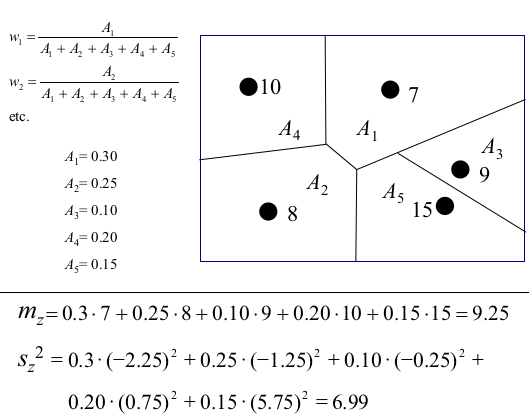
\includegraphics[width=\linewidth]{fiBi72.png}  % from Bierk
            \end{center}
\end{minipage}
\end{frame}

\begin{frame}{Descriptive spatial statistics}
    \begin{block}{Declustering}
    \end{block}
    \begin{itemize}
        \item The idea is to draw \alert{Thiessen polygons} around the observation locations first: by this procedure each location of the field is assigned to the closest observation.
        \item The relative sizes of the \emph{Thiessen polygons} are used as \emph{declustering weights}: $w_i = \frac{A_i}{\sum_j A_j}$.
        \item Using these weights the \emph{declustered histogram} and \emph{cumulative frequency distribution} can be calculated as shown in the figure below, as well as the \emph{declustered moments} such as the \emph{mean} and \emph{variance}:
\begin{minipage}[]{0.46\textwidth}
            \begin{equation}
                m_z = \sum_{i=1}^n w_i z_i
                \label{e71}
            \end{equation}
\end{minipage}
\hfill
\begin{minipage}[]{0.46\textwidth}
            \begin{equation}
                s_z^2 = \sum_{i=1}^n w_i (z_i-m_z)^2
                \label{e72}
            \end{equation}
\end{minipage}
            
            \vspace{-2pt}

\begin{minipage}[]{0.45\textwidth}
    \centering
            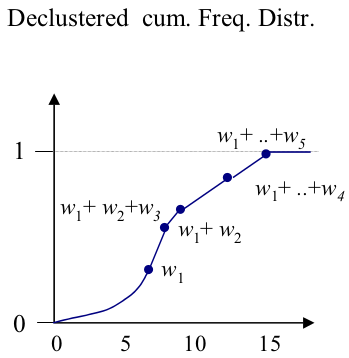
\includegraphics[width=0.8\linewidth]{fiBi73a.png}  % from Bierk
\end{minipage}
\hfill
\begin{minipage}[]{0.45\textwidth}
            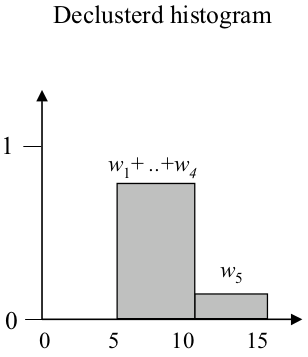
\includegraphics[width=0.8\linewidth]{fiBi73b.png}  % from Bierk
\end{minipage}

    \end{itemize}
\end{frame}

\begin{frame}{Descriptive spatial statistics}
    \begin{block}{Declustering}
    \end{block}
    \begin{itemize}
        \item The effect of \emph{declustering} can be demonstrated using the synthetithe data-set shown in the figure below (all of the larger numerical examples shown in here are based on this data set).

\begin{minipage}[]{0.45\textwidth}
    \centering
            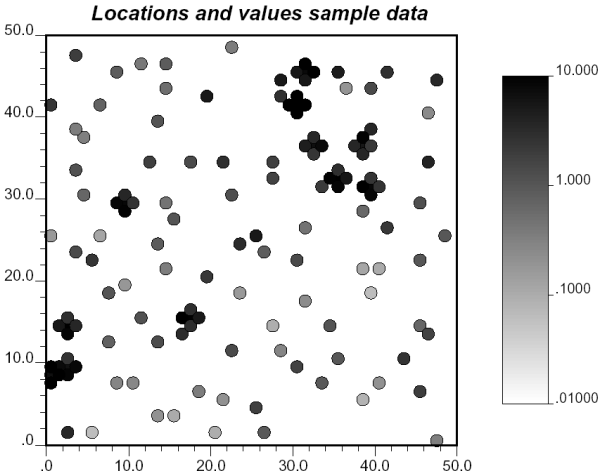
\includegraphics[width=\linewidth]{fiBi21.png}  % from Bierk
\end{minipage}
\hfill
\begin{minipage}[]{0.45\textwidth}
            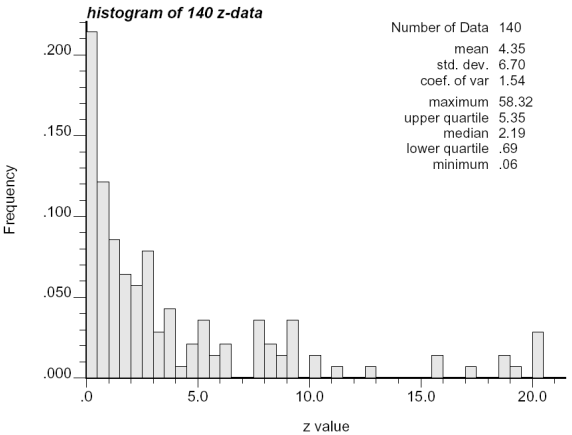
\includegraphics[width=\linewidth]{fiBi22.png}  % from Bierk
\end{minipage}

    \end{itemize}
\end{frame}

\begin{frame}{Descriptive spatial statistics}
    \begin{block}{Declustering}
    \end{block}
    \begin{itemize}
        \item The figure below shows the \emph{declusterd histogram} based on the 140 data and the \emph{”true” histogram } based on 2500 values.Clearly, the are very much alike, while the histogram based on the non-weighted data (see figure) is much different.
            \begin{center}
            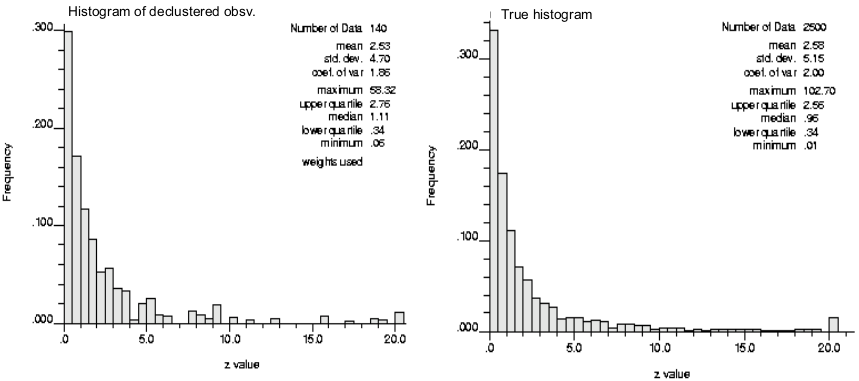
\includegraphics[width=\linewidth]{fiBi74.png}  % from Bierk
            \end{center}
        \item The estimated \emph{mean} without weighting equals 4.35 which is
much too large. The reason is the existance of clusters with very high data values present in the observations (see figure above).
\item \emph{Declustering} can correct for this as can be seen from the \emph{declustered mean} in the figure above which is 2.53 and very close to te true mean of 2.58.

    \end{itemize}
\end{frame}

\begin{frame}{Descriptive spatial statistics}
    \begin{block}{Semivariance and correlation}
    \end{block}
    \begin{itemize}
        \item Using the synthetic data set of 140 observations we will further illustate the concept of the \emph{semivariogram} and the \emph{correlation function}.
        \item Figure below shows scatter plots of the $z(\mathbf{x})$ and $z(\mathbf{x}+\mathbf{h})$ for  $|\mathbf{h}|= 1, 5, 10, 20$ units (pixels) apart. For each pair of points the distance $d_i$ to the one-to-one line it can be calculated.
            \begin{center}
            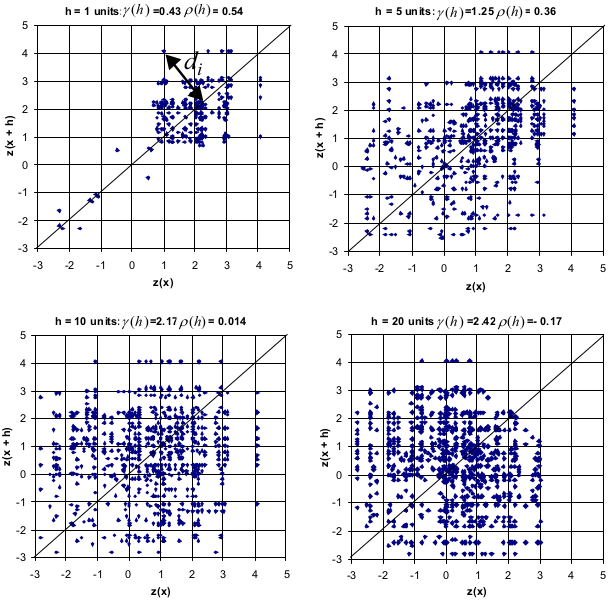
\includegraphics[width=0.6\linewidth]{fiBi75.png}  % from Bierk
            \end{center}
    \end{itemize}
\end{frame}

\begin{frame}{Descriptive spatial statistics}
            \vspace{-4pt}
    \begin{block}{Semivariance and correlation}
    \end{block}
            \vspace{-5pt}
    \begin{itemize}
        \item The \emph{semivariance} of a given distance is given by (with $n(h)$ the number of pairs of points that are a distance $h= |\mathbf{h}|$ apart)
            \vspace{-5pt}
            \begin{equation}
                \hat{\gamma} (h) = \frac{1}{2n(h)} \sum_{i=1}^{n(h)} d_i^2 = \frac{1}{2n(h)}\sum_{i=1}^{n(h)} \left[ z(\mathbf{x} + \mathbf{h})-z(\mathbf{x})\right]^2 
                \label{e73}
            \end{equation}
            and the \emph{correlation coefficient} 
            \vspace{-5pt}
            \begin{equation}
                \hat{\rho} (h) =  \frac{1}{n(h)}\sum_{i=1}^{n(h)} \frac{ z(\mathbf{x} + \mathbf{h})z(\mathbf{x}) - m_{z(\mathbf{x} + \mathbf{h})}  m_{z(\mathbf{x})}}{S_{z(\mathbf{x} + \mathbf{h})}  S_{z(\mathbf{x})}}
                \label{e74}
            \end{equation}
            $m_{z(\mathbf{x} + \mathbf{h})}$,  $m_{z(\mathbf{x})}$ and $S_{z(\mathbf{x} + \mathbf{h})}$,  $S_{z(\mathbf{x})}$ are the \emph{mean} and \emph{variance}  of the $z(\mathbf{x}+\mathbf{h})$ and $z(\mathbf{x})$ data values respectively. The figure below shows plots of the \emph{semivariance} and the \emph{correlation} as a function of distance.
            \begin{center}
            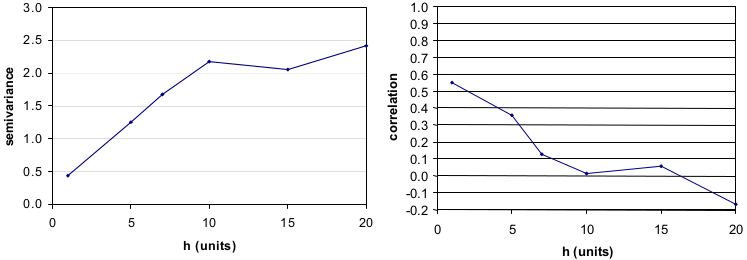
\includegraphics[width=0.8\linewidth]{fiBi76.png}  % from Bierk
            \end{center}
            \vspace{-5pt}
        \item These plots are called the \emph{semivariogram} and the \emph{correlogram} respectively. If we imagine the data $z$ to be observations from a realisation of a random function $Z(\mathbf{x})$ and this random function is assumed to be intrinsic or wide sense \emph{stationary}  then equations~\ref{e73} and ~\ref{e74} are estimators for the \emph{semivariance function} and the \emph{correlation function}.
    \end{itemize}
\end{frame}

%-------
% From Bierkens
\section{Spatial interpolation by kriging}
\begin{frame}{Spatial interpolation by kriging}
    \begin{block}{Generalities}
    \end{block}
    \begin{itemize}
        \item \alert{Kriging} is a collection of methods that can be used for \emph{spatial interpolation}.
        \item \alert{Kriging} provides \emph{optimal linear predictions} at non-observed locations by assuming that the unknown \emph{spatial variation} of the property is a realisation of a \emph{random function} that has been observed at the data points only.
        \item Apart from the prediction, \emph{kriging} also provides the \emph{variance} of the prediction
        \item Two \emph{kriging} variants are discussed: \alert{simple kriging} and \alert{ordinary kriging} which are based on slightly different \emph{random function} models.
    \end{itemize}
\end{frame}

\begin{frame}{Spatial interpolation by kriging}
    \begin{block}{Simple kriging}
    \end{block}
    The most elementary of \emph{kriging methods} is called \alert{simple kriging} and  is based on a \emph{random function} that is \emph{wide sense stationary}, i.e. with the following properties
    \begin{align*}
        E[Z(\mathbf{x})] &= \mu_Z = \text{ constant}\\
        var[Z(\mathbf{x})] &= E[Z(\mathbf{x})-\mu_Z ]^2 = \sigma_Z^2 = \text{ constant (and finite)}\\
        COV\left[Z(\mathbf{x}_1), Z(\mathbf{x}_2)\right] &= E\left[ (Z(\mathbf{x}_1)-\mu_Z )  (Z(\mathbf{x}_2)-\mu_Z )\right] = C_Z (\mathbf{x}_2 - \mathbf{x}_1 ) = C(\mathbf{h})
    \end{align*}
    \emph{Simple kriging} is the appropriate \emph{kriging method} if the \emph{random forest} is \emph{second order stationary} and the \emph{mean} of the \emph{random forest} $E[Z(\mathbf{x})] = \mu$ is known without error. With \emph{simple kriging} a predictor $\hat{Z}(\mathbf{x}_0)$ is sought that
    \begin{enumerate}
        \item is a linear function of the surrounding data,
        \item is unbiased: $E[\hat{Z}(\mathbf{x}_0)- Z(\mathbf{x}_0) ] = 0$,
        \item and has the smallest possible error, i.e. $\hat{Z}(\mathbf{x}_0) - Z(\mathbf{x}_0)$ is minimal.
    \end{enumerate}
    A \emph{linear} and \emph{unbiased} predictor is obtained when considering the following \emph{weighted average} of deviations from the \emph{mean}:
            \begin{equation}
                \hat{Z}(\mathbf{x}_0) = \mu_Z + \sum_{i=1}^n \lambda_i [Z(\mathbf{x}_i)-\mu_Z]
                \label{e75}
            \end{equation}
            with $Z(\mathbf{x}_i)$ the values of $Z(\mathbf{x})$ at the surrounding observation locations.

\end{frame}

 \begin{frame}{Spatial interpolation by kriging}
    \begin{block}{Simple kriging}
    \end{block}
    Usually, not all observed locations are included in the predictor, but only a limited number of locations within a given \emph{search neighbourhood}. Equation~\ref{e75} is unbiased by definition:
            \begin{equation}
                E[\hat{Z}(\mathbf{x}_0) -Z(\mathbf{x}_0)]  = \mu_Z + \sum_{i=1}^n \lambda_i [Z(\mathbf{x}_i)-\mu_Z] -E[Z(\mathbf{x}_0)] = \mu_Z + \sum_{i=1}^n \lambda_i [\mu_Z -\mu_Z] -\mu_Z = 0
                \label{e76}
            \end{equation}
            The \emph{weights} $\lambda_i$  should be chosen such that the \emph{prediction error} is minimal. However, as the real value $z(\mathbf{x}_0)$ is unknown, we cannot calculate the \emph{prediction error}. Therefore, instead of minimizing the prediction error we must be satisfied with minimizing the \emph{variance} of the prediction error $var[\hat{Z}(\mathbf{x}_0)-Z(\mathbf{x}_0)]$. Because the predictor is unbiased, the \emph{variance} of the \emph{prediction error} can be written as
            \begin{equation}
                \begin{aligned}
                &var[\hat{Z}(\mathbf{x}_0) -Z(\mathbf{x}_0)]  = E[\hat{Z}(\mathbf{x}_0) -Z(\mathbf{x}_0)]^2 = \\
                &E\left[  \sum_{i=1}^n \lambda_i E[Z(\mathbf{x}_i)-\mu_Z] -[Z(\mathbf{x}_0) -\mu_Z]\right]^2 = \\
                &\sum_{i=1}^n \sum_{j=1}^n  \lambda_i \lambda_j E\left[[Z(\mathbf{x}_i)-\mu_Z]  [Z(\mathbf{x}_j)-\mu_Z] \right] - \\
                &2\sum_{i=1}^n \lambda_i E\left[[Z(\mathbf{x}_i)-\mu_Z] [Z(\mathbf{x}_0)-\mu_Z] \right] + E[Z(\mathbf{x}_0)-\mu_z]^2
                \end{aligned}
                \label{e77}
            \end{equation}
\end{frame}
 
 \begin{frame}{Spatial interpolation by kriging}
    \begin{block}{Simple kriging}
    \end{block}
    Using the definition of the \emph{covariance} of a \emph{second order stationary stochastic field} $E\left[[Z(\mathbf{x}_i)-\mu_Z]  [Z(\mathbf{x}_j)-\mu_Z] \right] = C_Z(\mathbf{x}_i - \mathbf{x}_j )$ and $C_Z(0) =\sigma_Z^2$ , we obtain for the \emph{variance} of the \emph{prediction error}

            \begin{equation}
                var[\hat{Z}(\mathbf{x}_0) -Z(\mathbf{x}_0)]  = \sum_{i=1}^n \sum_{j=1}^n \lambda_i \lambda_j C_Z(\mathbf{x}_i - \mathbf{x}_j) - 2\sum_{i=1}^n \lambda_i C_Z(\mathbf{x}_i - \mathbf{x}_0) + \sigma_Z^2
                \label{e78}
            \end{equation}
            To obtain the minimum value of Equation~\ref{e78} we have to equate all its partial derivatives with respect to the $\lambda_i$ to zero:
            \begin{equation}
                \frac{\partial}{\partial \lambda_i} var[\hat{Z}(\mathbf{x}_0)- Z(\mathbf{x}_0)] = 2 \sum_{j=1}^n \lambda_j C_Z(\mathbf{x}_i-\mathbf{x}_j)-2C_Z (\mathbf{x}_i - \mathbf{x}_0 ) = 0 \quad \quad i=1,2,\cdots,n
                \label{e79}
            \end{equation}
            This results in the following system of $n$ equations referred to as the \alert{simple kriging system}
            \vspace{-5pt}
            \begin{equation}
                \sum_{j=1}^n \lambda_j C_Z (\mathbf{x}_i -\mathbf{x}_j) = C_Z (\mathbf{x}_i-\mathbf{x}_0) \quad \quad i=1,2,\cdots,n
                \label{e710}
            \end{equation}
            The $n$ unknown values $\lambda_i$ can be uniquely solved from these $n$ equations if all the $\mathbf{x}_i$ are different. The predictor in equation~\ref{e75} with the $\lambda_i$ found from solving equations~\ref{e710} is the one with the minimum \emph{prediction error variance}. This \emph{variance} can be calculated using equation~\ref{e78}. However, it can be shown that the \emph{variance} of the \emph{prediction error} can be written in a simpler form as
            \vspace{-5pt}
            \begin{equation}
                var[\hat{Z}(\mathbf{x}_0)- Z(\mathbf{x}_0)] = \sigma_Z^2 - \sum_{i=1}^n \lambda_i C_Z(\mathbf{x}_i - \mathbf{x}_0)
                \label{e711}
            \end{equation}

\end{frame}

 \begin{frame}{Spatial interpolation by kriging}
    \begin{block}{Simple kriging}
    \end{block}
    The \emph{error variance} very nicely shows how \emph{kriging} takes advantage of the spatial dependence of $Z(\mathbf{x}_i)$. If only the \emph{marginal probability distribution} had been estimated from the data and the spatial coordinates had not been taken into account, the best prediction for every non-observed location would have been the \emph{mean} $\mu_Z$. Consequently, the \emph{variance} of the \emph{prediction error} would have been equal to $\sigma_Z^2$. As the larger \emph{kriging weights} are positive, it can be seen from equation~\ref{e711} that the \emph{prediction error variance} of the \emph{kriging predictor} is always smaller than the variance of the \emph{random function}.

    To obtain a \emph{positive error variance} using equation~\ref{e711} the function $C(\mathbf{h})$ must be \emph{positive definite}. This means that for all possible $\mathbf{x}_1,\cdots,\mathbf{x}_n \in \Re^N \ (N=1,2\ or\ 3)$ and for all $\lambda_1, \lambda_2, \cdots, \lambda_n \in \Re$ the following inequality must hold
            \begin{equation}
                \sum_{i=1}^n \sum_{j=1}^n \lambda_i \lambda_j C_Z (\mathbf{x}_i - \mathbf{x}_j ) > 0
                \label{e712}
            \end{equation}
            \begin{itemize}
                \item It is difficult to ensure that this is the case for any \emph{covariance function}. Therefore, we cannot just estimate a \emph{covariance function} directly from the data for a limited number of separation distances and then obtain a \emph{continuous function} by \emph{linear interpolation} between the experimental points (such as in figure above). 
                \item If such a \emph{covariance function} were used in equation~\ref{e710}, equation~\ref{e711} would not necessarily lead to a positive estimate of the \emph{prediction error variance}. 
            \end{itemize}
\end{frame}

 \begin{frame}{Spatial interpolation by kriging}
    \begin{block}{Simple kriging}
    \end{block}
            \begin{itemize}
                \item In fact, there are only a limited number of functions for which it is proven that inequality~\ref{e712} will always hold. So the practical solution used in \emph{kriging} is to take one of these ‘permissible’ functions and fit it through the points of the experimental \emph{covariance function}. 
                \item Next, the values of the fitted function are used to build the \emph{kriging system} (see equation~\ref{e710} and to estimate the kriging variance using equation~\ref{e711}.
                \item The table below gives a number of \emph{covariance functions} that can be used for simple \emph{kriging} (i.e. using a wide sense stationary random functions).Of course, in case of second order stationarity the parameter $c$ should be equal to the \emph{variance} of the random function: $c = \sigma_Z^2$.
    \begin{center}
  \begin{tabular}{|l|c|}
    Exponential covariance & $C_Z (h) = c e^{-h/a}$ for $h\geq 0$, $a>0$ \\ 
    Gaussian covariance         & $C_Z (h) =  c  e^{-h^2 / a^2}$  for $h\geq 0$, $a>0$ \\ 
    Spherical covariance         & $ C_Z (h) = \left\{ \begin{array}{l}  c \left[ 1 - \frac{3}{2}\left(\frac{h}{a}\right) + \frac{1}{2}\left(\frac{h}{a}\right)^3 \right]   \text{, if } h< a  \\ 0 = \text{, if } h\geq a, h\geq 0, a>0 \end{array} \right. $ \\ 
    Nugget model &  $ \rho_Z (h) = \left\{ \begin{array}{l}  c \text{, if } h=0  \\ 0 = \text{, if } h>0 \end{array} \right. $ \\ 
  \end{tabular}
    \end{center}
            \end{itemize}
    \end{frame}

 \begin{frame}{Spatial interpolation by kriging}
    \begin{block}{Simple kriging}
    \end{block}
    \begin{itemize}
        \item The figure below shows an example of an \emph{exponential model} that is fitted to the \emph{estimated covariances}.

            \begin{center}
            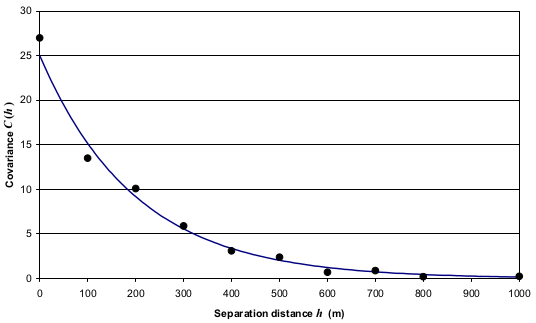
\includegraphics[width=0.7\linewidth]{fiBi77.png}  % from Bierk
            \end{center}
%         \item Some remarks should be made about the \emph{nugget model}.
%             \begin{itemize}
%                 \item The nugget stems from the mining practice. Imagine that we find occasional gold nuggets in surrounding rock that doesn’t contain any gold itself. If we were to estimate the covariance function of gold content from our
% observation, we would get the nugget model with c   2Z  p1  p (with p the probability of
% finding a gold nugget).
        \item Any linear combination of a \emph{permissible covariance model} is a permissible covariance model itself. Often a combination of a \emph{nugget model} and another model is observed, e.g:
            \vspace{-5pt}
            \begin{equation}
                C (h) = \left\{ \begin{array}{l}  c_0 + c_1  \text{, if } h= 0  \\ c_1 e^{-h/a} \text{, if }  h > 0 \end{array} \right. 
                \label{e711}
            \end{equation}
            where $c_0 + c_1 = \sigma_Z^2$. In this case $c_0$ is often used to model the part of the variance that is attributable to \emph{observation errors} or \emph{spatial variation} that occurs at distances smaller than the minimal distance between observations.


    \end{itemize}
    \end{frame}
\end{document}



